\scanpage{24}
\mspage{11}
it is a locally constant function on $\mathcal S$.

Let us fix an \inserted{\uline{anabelian} $(2g+\nu\geq3)$} numerical type $(g,\nu)$, and consider, for variable $\mathcal S$, the fibered groupoid
\[
(24)\qquad\mathcal S\longmapsto\widehat{M}_{g,\nu}(\mathcal S)=\begin{gathered}\text{Mumford-Deligne curves}\\\text{\unsure{relative|relives} over }\mathcal S,\text{ of}\\\text{numerical type}\\\text{equal \unsure{to|:} }(g,\nu)\end{gathered}
\]
We then have the following truly marvellous theorem:

\margin{We \unsure{suppose|supp\textsuperscript{ose}} $2g+\nu\geq3$ (anabelian case)}
\uline{Theorem} of \uline{Mumford-Deligne}: The

\figure{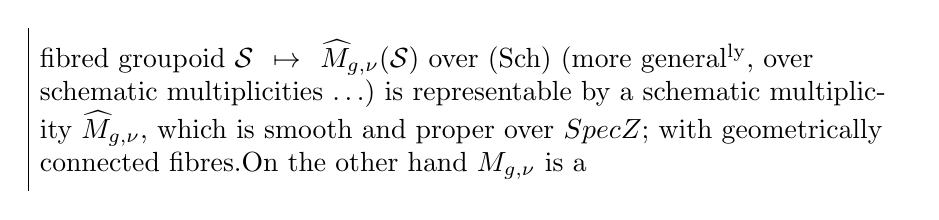
\begin{tikzpicture}
\node[anchor=north west,text width=0.9\linewidth,align=left,inner sep=4pt] (T) at (0,0) {
fibred groupoid $\mathcal S\mapsto\widehat{M}_{g,\nu}(\mathcal S)$ over $(\mathrm{Sch})$ (more general\textsuperscript{ly}, over schematic multiplicities $\ldots$) is representable by a schematic multiplicity $\widehat{M}_{g,\nu}$, which is \uline{smooth} and \uline{proper} over $\operatorname{Spec}\mathbb Z$; \deleted{with geometrically connected fibres.}\inserted{On the other hand $M_{g,\nu}$ is a}
};
\draw[line width=0.5pt] (T.north west)--(T.south west);
\end{tikzpicture}}
\mspage{23}
